\documentclass[12pt]{article}
\usepackage[margin=1in]{geometry}
\usepackage{fontspec}
\setmainfont{Times New Roman}
\usepackage[utf8]{inputenc}
\usepackage{graphicx} 
\usepackage{float} 
\usepackage{amsmath} 
\usepackage{subfigure}
\usepackage{booktabs}
\usepackage[singlespacing]{setspace}
\title{\vspace{-1.0cm}STAT628 Module2 Group20}
\author{Yuanhao Geng, Yuxin Zhao, Mingyu Wang, Jiayang Wang}
\date{}

\setlength\parindent{0pt}

\begin{document}

\maketitle
\vspace{-1.5cm}
\section{\vspace{-0.3cm}Introduction and Background}
In this program, we get a body fat dataset of 252 men with measurements of their percentage of body fat and 14 different body circumference measurements like Neck circumference, etc. We use lasso and stepwise regression to select explanatory feature respectively, then use MSE as the criterion to choose model. The R-square of our final model is 0.735.
\vspace{-0.6cm}
\section{\vspace{-0.3cm}Data Cleaning}

Here we use the empirical method Siri's equation: $\rm Fat=\frac{495}{Density} - 450$, where density is measured under water and should be bounded within $(0.9,1.1)$. Therefore, we delete individual IDNO 182 whose body density is 1.1089. From the scatter plot of body fat and density, we found there are 3 obvious outliers out of the ideal line. Then we use the Siri's equation to compute the estimated body fat and substract it by the corresponding original BODYFAT in dataset to get errors. The distribution of error is nearly a normal distribution with mean 0. Then we use $3\sigma$ criterion to find out these outliers successfully. Finally, we impute the body fat of these three individuals IDNO 48, 76, 96 by estimated body fat from Siri's equation.
\vspace{-0.6cm}
\section{\vspace{-0.3cm}Feature Selection}

Here we consider 2 methods for the feature selection step: LASSO and stepwise regression.
LASSO is use $L_1$ norm to keep the sparsity of the estimated solution. The features with non-zero coefficient are selected to be the important variables. Finally, we select four features: Weight, Height, Abdomen and Thigh.
For the stepwise regression, the process consists of two basic steps: one is to remove variables from the regression model that are not significant by t-test, and the other is to introduce new variables into the regression model that are significant by F-test. Here, we set both thresholds for introducing and removing variables as $0.05$. Finally, we select four features: Weight, Wrist, Abdomen and Forearm.
\vspace{-0.6cm}
\section{\vspace{-0.3cm}Model}
%\subsection{Choosing Model}
We use both R-square and mean square error on test set to choose out final model. From the table below, we found that the stepwise regression model performs better both on training set and test set. The R-square of the stepwise model is larger than the lasso one and the MSE on test error is smaller so that its generalization ability is better.

\begin{center}
\begin{tabular}{ c c c}
\hline
  model & lasso model & stepwise regression \\ 
   \hline
 R-square & 0.7245 & 0.7351 \\  
  \hline
 MSE on test set &18.228  & 17.208\\
  \hline
\end{tabular}
\end{center}
%\vspace{-0.6cm}
%\subsection{\vspace{-0.3cm}Final Model and Interpretation}
Our final model is a linear regression model based on the stepwise regression above, which is $y = -31.30 + 0.92x_1 -1.39x_2 +0.45x_3 -0.13x_4$, where y is percentage of the body fat in the adult men, $x_1$ is abdomen, $x_2$ is wrist, $x_3$ is forearm and $x_4$ is weight. This means that if a man with 90cm of abdomen 2 circumference, 18cm of wrist circumference, 170lbs of weight and 26 cm of forearm circumference then is expected to have a body fat percent of 16.83.This means that assuming other factors remain constant, every abdomen circumference increase in 1cm, the model predicts that the body fat percent will increase, on average, by 0.92 and the 1cm increase of forearm circumference will lead to 0.44 increase of body fat percentage.
\newline

%\vspace{-0.6cm}
%\subsection{\vspace{-0.3cm}Statistical Analysis}
We separately conduct T-test to see whether the predictor we have chosen is related to the response and we got all p-values are below 0.05 which is the significance level we chose. Then we conduct the overall F-test and the F-statistics is 171.4 which is much larger than 1, so it provides compelling evidence suggests against the null hypothesis.
\vspace{-0.6cm}
\section{\vspace{-0.3cm}Model Diagnostics}

We checked the following four assumptions (linearity, homoskedasticity, independence, normality) for SLR. First, we checked linearity, homoskedasticity and independence using Residual Plot (see Figure 1). We see a random-looking, equal distribution of points on both sides of x axis, so we believe linearity, homoskedasticity and independence are plausible, even though there is slight violations of large fitted values. 
Second, we checked normality using QQ Plot (see Figure 2). We see the points in a QQ plot approximately lie on a straight diagonal line with some violations. Therefore, we decide to use the Shapiro-Wilk test to test normality precisely. According to the result of Shapiro-Wilk test, we fail to reject 'the sample is normal' because p-value is 0.06 (0.05935) higher than 0.05. All in all, these four assumptions are all valid according to reasons above.

\begin{figure}[H]
\centering
\begin{minipage}[t]{0.4\textwidth}
\centering
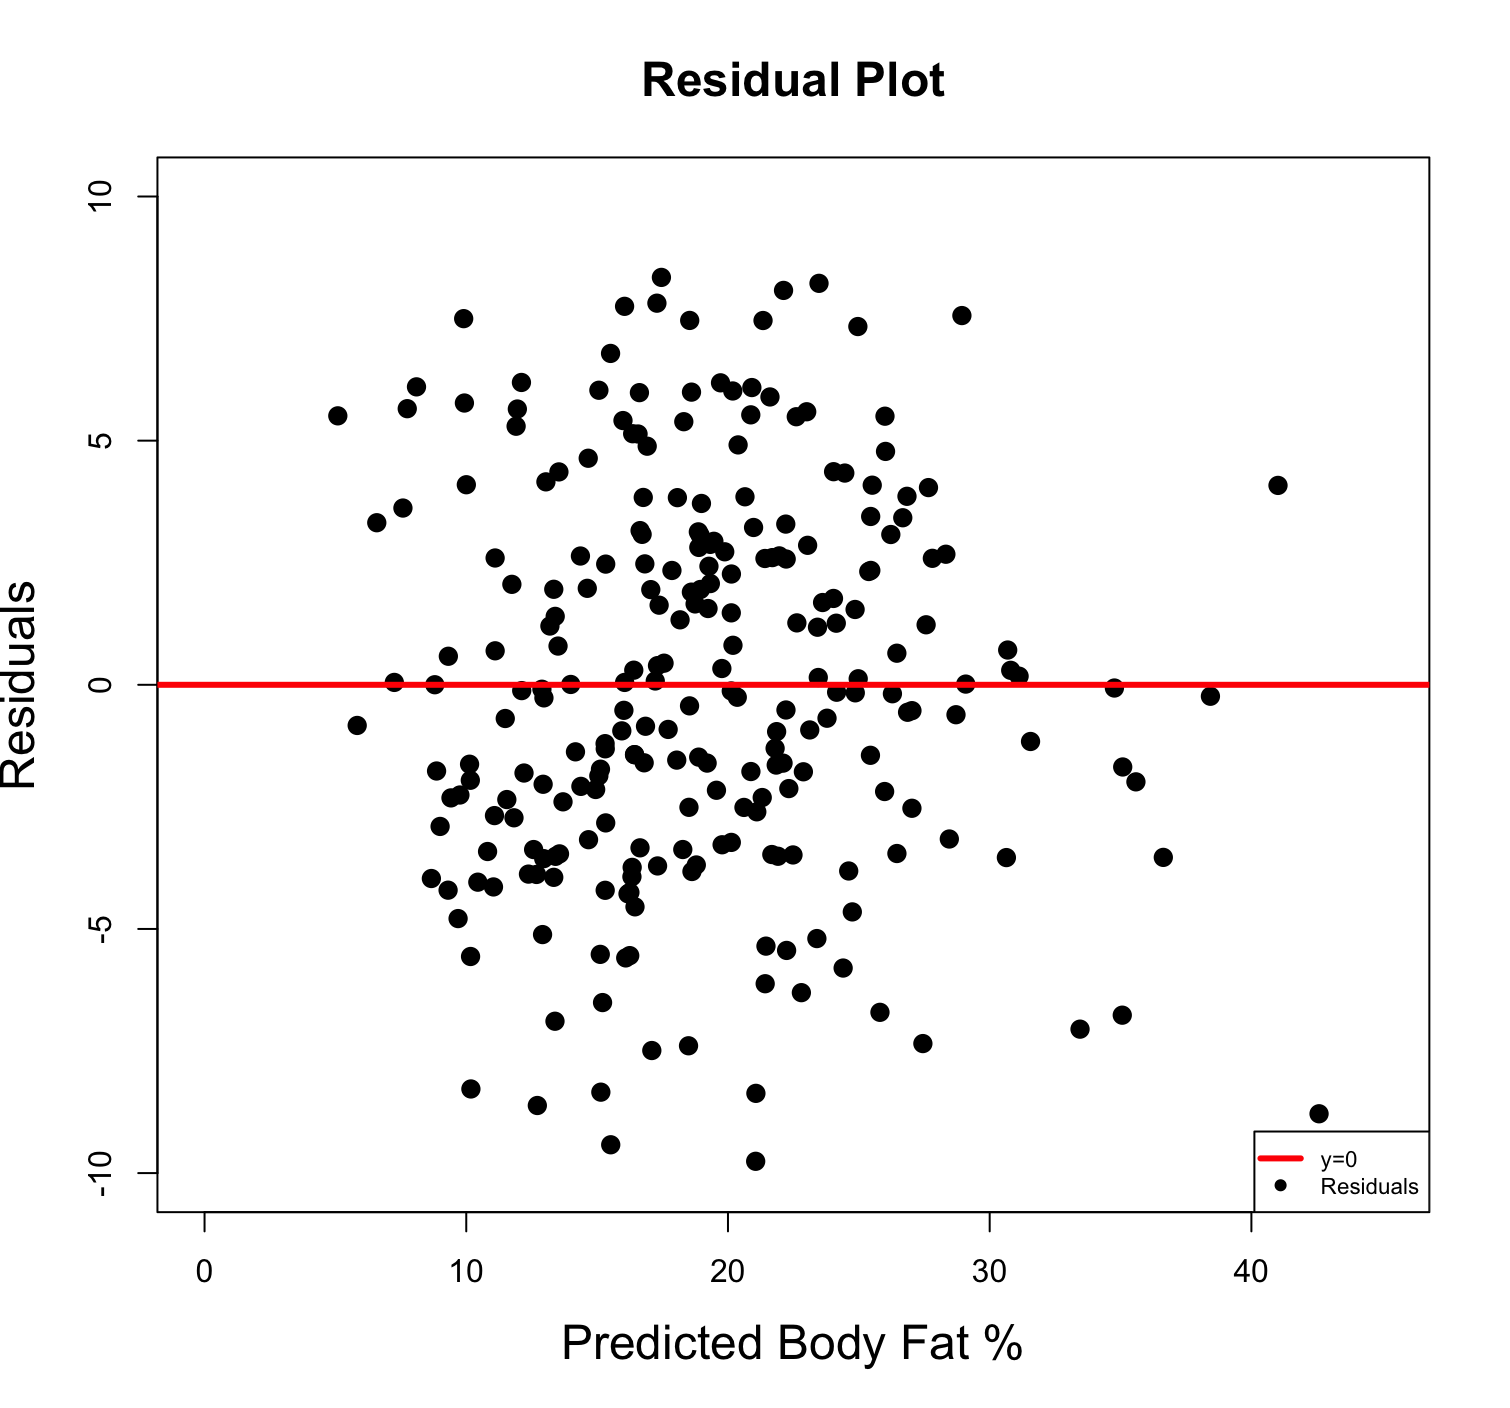
\includegraphics[width=4.5cm]{../image/residual_plot.png}
\caption{Residual Plot}
\end{minipage}
\begin{minipage}[t]{0.4\textwidth}
\centering
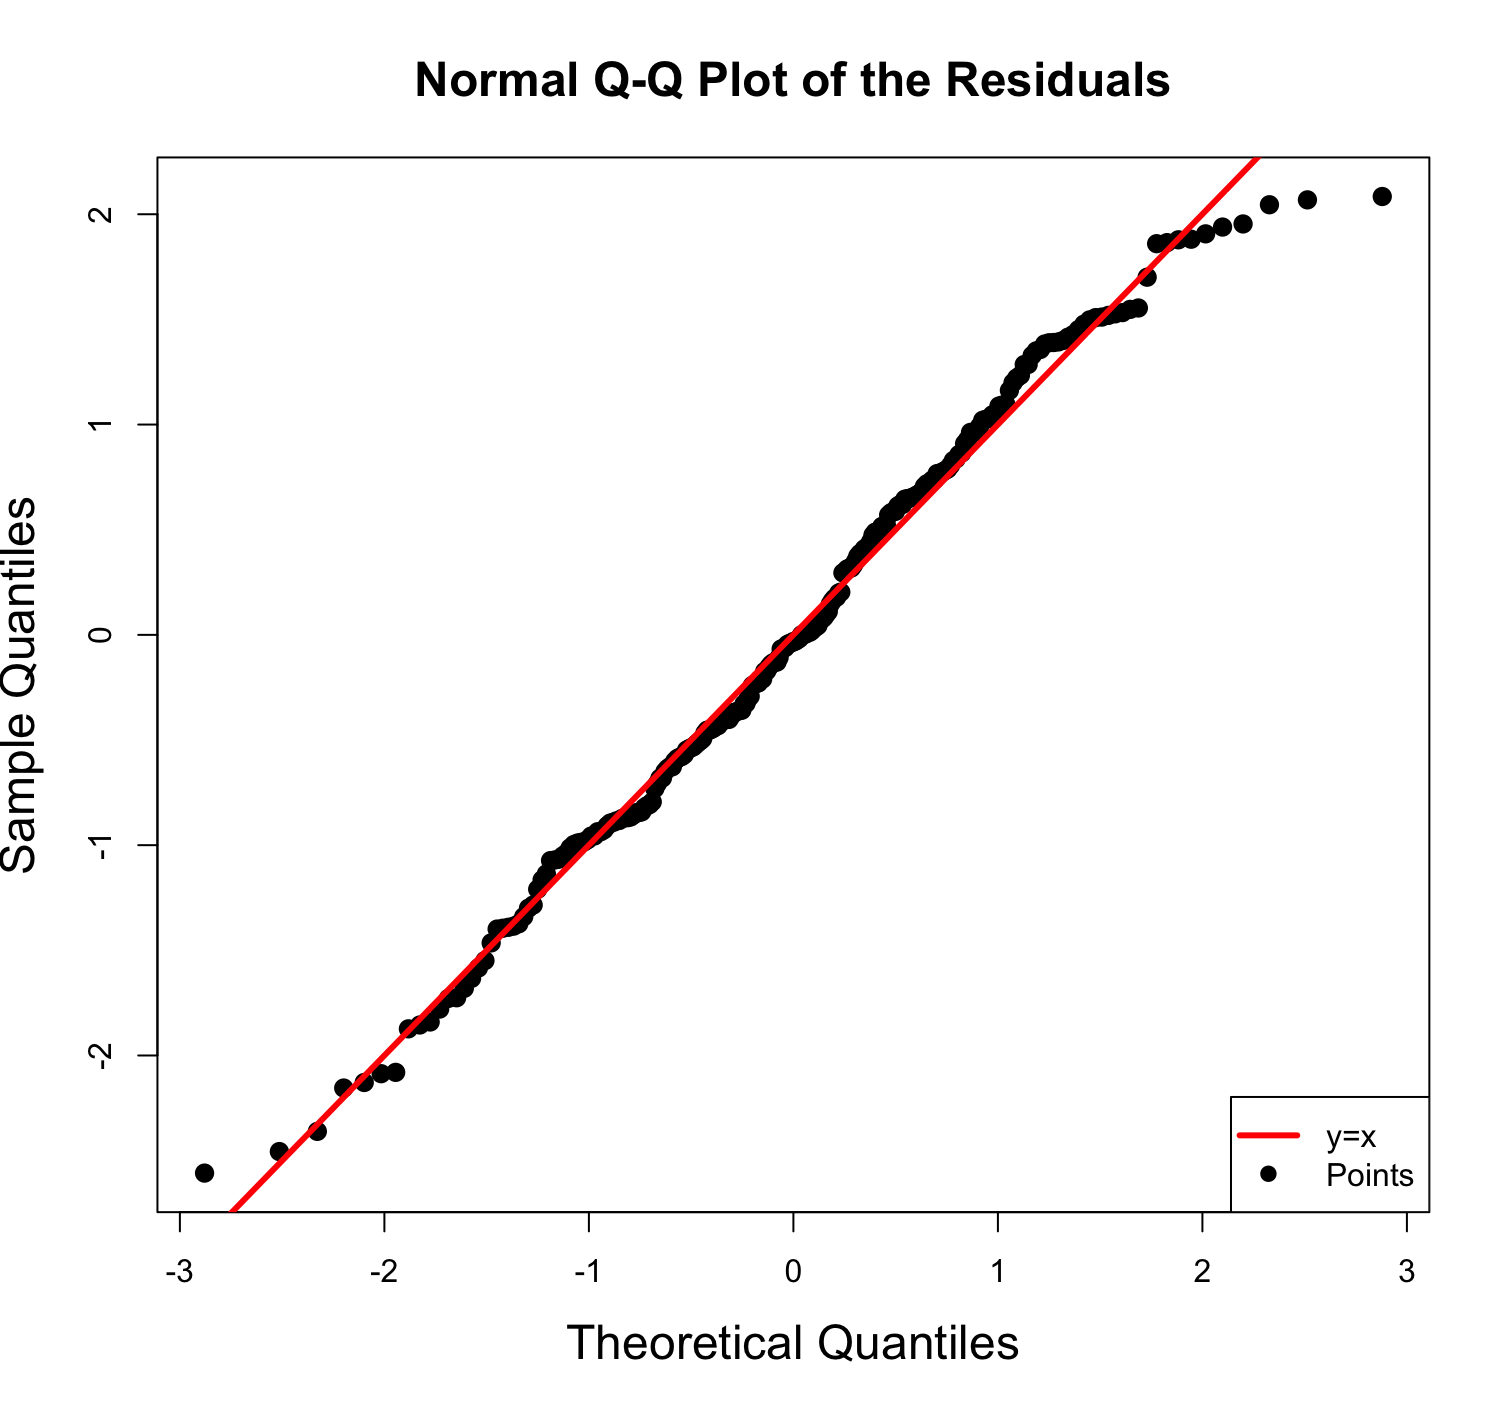
\includegraphics[width=4.5cm]{../image/QQ_plot.png}
\caption{QQ Plot}
\end{minipage}
\end{figure}

% \begin{figure}[htbp]
% \centering
% \begin{minipage}[t]{0.48\textwidth}
% \centering
% \includegraphics[width=6cm]{Independence.png}
% \caption{Test of Independence Residual Plot}
% \end{minipage}
% \begin{minipage}[t]{0.48\textwidth}
% \centering
% 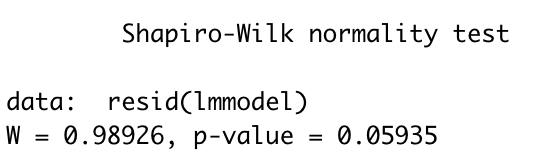
\includegraphics[width=6cm]{Nomality.png}
% \caption{Shapiro-Wilk test}
% \end{minipage}
% \end{figure}
\vspace{-1.2cm}
\section{\vspace{-0.3cm}Model Strengths and Weakness}
As to the strength of the model, our model satisfies the linear regression assumption of homoskedasticity and linearity and it is explainable about its result. Meanwhile, the stepwise regression method overcomes the multiple linearity of predictors of the model. As to weakness, the final model contains 4 predictors, which is kind of complicated. Also, if a man has extreme values, the model may produce negative body fat prediction.

\vspace{-0.6cm}
\section{\vspace{-0.3cm}Conclusion}

In summary, in order to estimate percentage of body fat using clinically available measurements, we firstly used lasso and stepwise regression to select explanatory feature respectively, then used MSE as the criterion to choose Models. Still, we also met some problems like some prediction values are negative. In the future, some non-linear models can be used if we have more data.


\newpage
\section{\vspace{-0.3cm}Contributions}

\begin{itemize}
\item YZ wrote the model fitting and statistical intepration part of the summary, worked on slides on page 7 to page 9. YZ also created code related to the model performance measure and model building.
\item YG wrote the feature selection part of the summary, worked on slides on page 5 to page 6. YG also created code related to the feature selection and development the Streamlit App.
\item JW wrote the model diagnostic part of the summary, worked on slides 10 to 14. JW also created code related to model diagnostics, maintained the code related to Figure 1 and Figure 2, and is ultimately responsible for the model diagnostic portion of the code.
\item MW edited 2-4 pages for slides, 1 and 2 subsections for presentation and created code for data cleaning.
\end{itemize}

\end{document}
